\documentclass{article}

\usepackage[left=1in, right=1in, top=1in, bottom=1in]{geometry}

\usepackage{setspace}
\usepackage{fancyhdr}
\usepackage{hyperref}
\usepackage{amsthm}
\usepackage{amssymb}
\usepackage{multirow}
\usepackage{enumitem}
\usepackage{graphicx}
\usepackage{makecell}
\usepackage{booktabs}
\usepackage{titlesec}
\usepackage{amsmath}
\usepackage{pdfpages}

\setcounter{secnumdepth}{4}

\hypersetup{
    colorlinks=true,     
    urlcolor=magenta
}

\renewcommand{\qedsymbol}{\rule{0.7em}{0.7em}}

\newlength\tindent
\setlength{\tindent}{\parindent}
\setlength{\parindent}{0pt}
\renewcommand{\indent}{\hspace*{\tindent}}
\setlength{\parskip}{0em}

\newenvironment{blockquote}{%
  \par%
  \vskip1em
  \leftskip=2em\rightskip=2em%
  \noindent\ignorespaces}{%
  \par\vskip1em}

\newenvironment{blockquote2}{%
	\par%
	\vskip1em
	\leftskip=4em\rightskip=4em%
	\noindent\ignorespaces}{%
	\par\vskip1em}

\pagestyle{fancy}
\fancyhf{}
\fancyhead[LO]{STA5176}
\fancyhead[RO]{Kyle Ligon}
\fancyfoot[LO]{Chapter 7}
\fancyfoot[RO]{\thepage}
 
\renewcommand{\headrulewidth}{0.5pt}
\renewcommand{\footrulewidth}{0.5pt}

\begin{document}
\section*{Chapter 7 Homework}
\subsection*{Due 2-23-2018}
\subsubsection*{Problem 7.7}
\subsubsection*{ b) Estimate the variation in reading scores using a 99\% Confidence Interval}
Which Confidence Interval?
\begin{blockquote}
Since we are trying to estimate the variation in the reading scores with a Confidence Interval, we should use $100(1-\alpha)\%$ CI for $\sigma^{2}$ which involves $\chi^{2}$.  
\end{blockquote}

Assumptions:
\begin{blockquote}
1) The population distribution is normal.  
\end{blockquote}

Confidence Interval Equation:
\begin{blockquote}
The Confidence Interval for Variance is as follows:
\begin{eqnarray}
C.I. = \left(\frac{\left(n-1\right)s^{2}}{\chi_{U}^{2}}, \sigma^{2}, \frac{\left(n-1\right)s^{2}}{\chi_{L}^{2}}\right) \nonumber \\
C.I. = \left(\frac{\left(150 - 1\right)9.537^{2}}{147.2568}, \sigma^{2}, \frac{\left(150-1\right)9.537^{2}}{117.098}\right)  \nonumber \\
C.I. \approx \left(92.0311, \sigma^{2}, 115.7338 \right) \nonumber \\
\end{eqnarray}
\end{blockquote}

Conclusion/Interpretation:
\begin{blockquote}
We are 95\% confidence that the Variance in the reading scores in the large public school system is between 92.0311 and 115.7338 points.  
\end{blockquote}


\subsubsection*{c) Do the data indicate that the standard deviation in reading scores is greater than 9, the standard deviation for all students taking the exam the previous yea?  Use $\alpha$ = 0.01 in reaching your conclusion}
Hypotheses:
\begin{blockquote}
With this test wanting to compare the standard deviation of theses students scores to the previous year's statewide results, we will use a Statistical Test for $\sigma^{2}$ and compare it to the Statewide Variance from last year of 81. \\

$H_0: \sigma^{2} \leq \sigma_0^{2} = 81$ \\
$H_1: \sigma^{2} > \sigma_0^{2} = 81$\\

\end{blockquote}
Assumptions:
\begin{blockquote}
1) We will still be assuming the population distribution is normal.  
\end{blockquote}

Test Statistic:
\begin{blockquote}
In order to find out the results of our statistical test, we will find the value of $\chi^{2}$ to determine if we can reject the null hypothesis. 

\begin{eqnarray}
\chi_0^{2} = \frac{\left(n-1\right)s^{2}}{\sigma_0^{2}} \nonumber \\
\chi_0^{2} = \frac{\left(149\right)\left(9.537^{2}\right)}{9^{2}} \nonumber \\
\chi_0^{2} = 167.3111 \nonumber \\
\end{eqnarray}
\end{blockquote}

Rejection Region:
\begin{blockquote}
Since we have a one tail greater than test, if $\chi_0^{2} \geq \chi_{U}^{2}$, then we can reject the null hypothesis.  Using the qchisq function in R to get the upper bound, we have a $\chi_{U}^{2} = 192.073$  
\end{blockquote}

P-Value:
\begin{blockquote}
In order to get the P-value for chi-square value, we will utilize the R function pchisq.  Subtracting the value returned from 1 gives us a p-value of 0.1449.  
\end{blockquote}

Conclusion/Interpretation:
\begin{blockquote}
Since our $\chi_0^{2} < \chi_{U}^{2}$ and out p-value $> \alpha$, we do not have extreme enough results to reject the Null Hypothesis that the standard deviation of our group is less than or equal to the statewide performance last year.  
\end{blockquote}


\subsubsection*{Problem 7.16}
\subsubsection*{a) 95\% C.I. for $\frac{\sigma_1}{\sigma_2}$}
\begin{blockquote}
Assume the Computer Group as Group 1 and Conventional Group as Group 2.  Since we are estimating a ratio of variances at the 0.95 Confidence Level, we will use the following equation: 
\begin{eqnarray}
C.I. = \left(\sqrt{\frac{s_{1}^{2}}{s_{2}^{2}}F_{1-\frac{\alpha}{2}, n_2 - 1, n_1 - 1}}, \sqrt{\frac{s_1^{2}}{s_2^{2}}F_{\frac{\alpha}{2}, n_{2}-1, n_{1}-1}}\right) \nonumber \\
C.I. = \left(\sqrt{\frac{53.77^{2}}{36.94^{2}}\left(1.58\right)}, \sqrt{\frac{53.77^{2}}{36.94^{2}}\left(\frac{1}{1.58}\right)}\right) \nonumber \\
C.I. \approx \left(1.1580, 1.8300\right) \nonumber \\
\end{eqnarray}
\end{blockquote}
Conclusion/Interpretation:
\begin{blockquote}
We are 95\% confident the true ratio of standard deviation's between the Computer test taking group and the Conventional test taking group lie between 1.1580 and 1.8300.  
\end{blockquote}

\subsubsection*{b) Hypothesis test for $\sigma_1 = \sigma_2$; $\alpha$ = 0.05}
Hypotheses:
\begin{blockquote}
Since we want to check for equality amongst our standard deviations, we will use the statistical test for $\sigma_1^{2}$ and $\sigma_2^{2}$.  Group 1 will still be Computers, and Group 2 will be Conventional. \\
$H_0: \sigma_{Comp}^{2} = \sigma_{Conv}^{2}$ \\
$H_1: \sigma_{Comp}^{2} \neq \sigma_{Conv}^{2}$
\end{blockquote}
\pagebreak
Assumptions:
\begin{blockquote}
1) Samples come from normally distributed populations.  
\end{blockquote}

Test Statistic:
\begin{eqnarray}
F_0 = \frac{53.77^{2}}{36.94^{2}} \nonumber \\
F_0 = 2.1188 \nonumber \\
\end{eqnarray}


Rejection Region:
\begin{blockquote}
We are looking for both $F_{1-\frac{\alpha}{2}}$ and $F_{\frac{\alpha}{2}}$ to determine if the $H_0$ is in line for rejection.  Thus, by using the table, $F_{0.025}$ = $\frac{1}{1.53} = 0.6536$ and $F_{0.975} = 1.53$.  These will be the two values we will compare our 2.1188 to.  
\end{blockquote}

P-Value:
\begin{blockquote}
In order to arrive at the p-value for 2.1188 with $df_1$ and $df_2$ both being 90, we will utilize the pf function in R to get the appropriate p-value for our F statistic.  The function yields a cumulative probability to the left of 0.9997.  Thus, our p-value is 0.0003
\end{blockquote}

Conclusion/Interpretation:
\begin{blockquote}
Since our F statistic of 2.1188 is greater than our high end F Boundary of 1.53, there is sufficient evidence to reject the hypothesis that the population variances are equal.  We have extreme enough evidence to appear that the population variances are different between the group of students who took their exam on the computer and the group that took their test in a conventional method.  Using the p-value, we have evidence to point in the same direction.  This is because it is less than our $\frac{\alpha}{2}$ of 0.025. 
\linebreak
\indent Since $\sigma=\sqrt{\sigma^{2}}$, we can reject the null hypothesis that the standard deviations of the populations are not equal, and that evidence suggests that the population standard deviations are different.  
\end{blockquote}


\subsubsection*{c)95\% C.I. for $\mu_1 - \mu_2$}
Which Confidence Interval Should We Use?:
\begin{blockquote}
Due to the fact that we are dealing with unequal variances or unequal standard deviations, we are going to follow down the path of using Satterwaite's approximation of $\mu_{Comp}-\mu_{Conv}$.  
\end{blockquote}

Assumptions:
\begin{blockquote}
1) Independent Samples for both groups. \\
2) We are assuming unequal variances hold from the problem b)
\end{blockquote}

Confidence Interval Equation:
\begin{blockquote}
In order to complete Satterwhaitte's approximation, we must find our degrees of freedom.  They are found by using this equation:
\end{blockquote}
\begin{eqnarray}
df = \frac{\left(\frac{s_{Comp}^{2}}{n_{Comp}}+\frac{s_{Conv}^{2}}{n_{Conv}}\right)}{\frac{\left(\frac{s_{Comp}^{2}}{n_{Comp}}\right)^{2}}{n_{Comp}-1} + \frac{\left(\frac{s_{Conv}^{2}}{n_{Conv}}\right)^{2}}{n_{Conv}-1}} \nonumber \\
df = \frac{\left(\frac{53.77^{2}}{91}+\frac{36.94^{2}}{91}\right)}{\frac{\left(\frac{53.77^{2}}{91}\right)^{2}}{90} + \frac{\left(\frac{36.94^{2}}{91}\right)^{2}}{90}} \nonumber \\
df = \frac{31.7716 + 14.9952}{11.2159+2.4984} \nonumber \\
df = \frac{46.7668}{13.7143} \nonumber \\
df = 3.4101 \nonumber \\
df = 3 \nonumber
\end{eqnarray}
\begin{blockquote}
Now that we have our degrees of freedom, we can find the C.I. for the difference in the two means.  
\end{blockquote}
\begin{eqnarray}
C.I. = \left(\bar{y_{Comp}} - \bar{y_{Conv}}\right) \pm t_{\frac{\alpha}{2}, df}\sqrt{\frac{s_{Comp}^{2}}{n_{Comp}} + \frac{s_{Conv}^{2}}{n_{Conv}}} \nonumber \\
C.I. = \left(484.45 - 487.38\right) \pm 3.182\sqrt{\frac{53.77}{91}^{2}+\frac{36.94}{91}^{2}} \nonumber \\
C.I. = -2.93 \pm 3.182\sqrt{46.7668} \nonumber \\
C.I. = -2.93 \pm 90.1468 \nonumber \\
C.I. \approx \left(-93.0768, 87.2168\right) \nonumber \\
\end{eqnarray}
Conclusion/Interpretation:
\begin{blockquote}
We are 95\% confident that the difference in the mean SAT scores of the Computer group and Conventional test taking group is between -93.0768 and 87.2168.  
\end{blockquote}

\subsubsection*{d) Hypothesis test for $\mu_1 = \mu_2$; $\alpha$ = 0.05}
Hypotheses:
\begin{blockquote}
Since we are checking the means of the two groups to see if they're equal, we will use Satterwaite's approximation to find the differences since the variances are still unequal from part b).  \\
\indent $H_0: \mu_{Comp} - \mu_{Conv} = 0 $ \\
\indent $H_1: \mu_{Comp} - \mu_{Conv} \neq 0 $
\end{blockquote}
Assumptions:
\begin{blockquote}
1) Independent Samples \\
2) Unequal Variances \\
\end{blockquote}

Test Statistic:
\begin{eqnarray}
t_0 = \frac{\left(\bar{y_{Comp}}-\bar{y_{Conv}}\right) - D_0}{\sqrt{\frac{s_{Comp}^{2}}{n_{Comp}} + \frac{s_{Conv}^{2}}{n_{Conv}}}} \nonumber \\
t_0 = \frac{\left(484.45-487.38\right)-0}{\sqrt{\frac{53.77^{2}}{91}+\frac{36.94^{2}}{91}}} \nonumber \\
t_0 = \frac{-2.93}{\sqrt{46.7668}} \nonumber \\
t_0 = \frac{-2.93}{6.8386} \nonumber \\
t_0 = -0.4284 \nonumber 
\end{eqnarray}

Rejection Region:
\begin{blockquote}
In order to find the rejection boundary of our problem, we must check our  $t_{\frac{0.05}{2}, 3}$ .  The 3 came from the Satterwaite's df approximation above.  That t value = 3.182.     
\end{blockquote}

P-Value:
\begin{blockquote}
The p-value on a t score = -0.4284 is 0.3486.  This was derived from the pt function in R.    
\end{blockquote}

Conclusion/Interpretation:
\begin{blockquote}
Since our the absolute value of our Test Statistic is less than the t-value of our rejection bound of 3.182, there's not sufficient evident to reject the hypothesis that the two means are equal.  There does not seem to be evidence to suggest that the two group's mean scores are different.  
\end{blockquote}


\subsubsection*{Problem 7.18 }
\subsubsection*{a) Perform a BFL test using R; you must present results in usual hypothesis test format; $\alpha$ = 0.05}
Hypotheses:
\begin{blockquote}
Since there are multiple groups, we will be using the BFL test for multiple variances.  \\
$H_0: \sigma_W^{2} = \sigma_R^{2} = \sigma_Z^{2}$ \\
$H_1$: at least one of these variances are different
\end{blockquote}

Assumptions:
\begin{blockquote}
1) The assumptions for ANOVA on our transformed response variable hold.
\end{blockquote}

Test Statistic:
\begin{blockquote}
We will turn to R's lawstat package and the lavene function set around the median to get our test statistic.  In this case, our test statistic is F = 1.4392.  
\end{blockquote}

Rejection Region:
\begin{blockquote}
To find the boundary of our Rejection Region, we will look up our F statistic at $\alpha$, t - 1, N - t.  That $F_{0.05, 2, 21}$ statistic is 3.47.  
\end{blockquote}

P-value:
\begin{blockquote}
Just like we got our test stat from R's 'lavene' function centered around the median, we will also get the p-value from there as well.  The p-value is 0.2596.  
\end{blockquote}

Conclusion/Interpretation:
\begin{blockquote}
Since our p-value is larger than 0.05 and our test statistic is less than the rejection region, we do not have extreme enough data to reject the hypothesis that the variances are equal.  It does not appear that at least one of the variances is different.  
\end{blockquote}

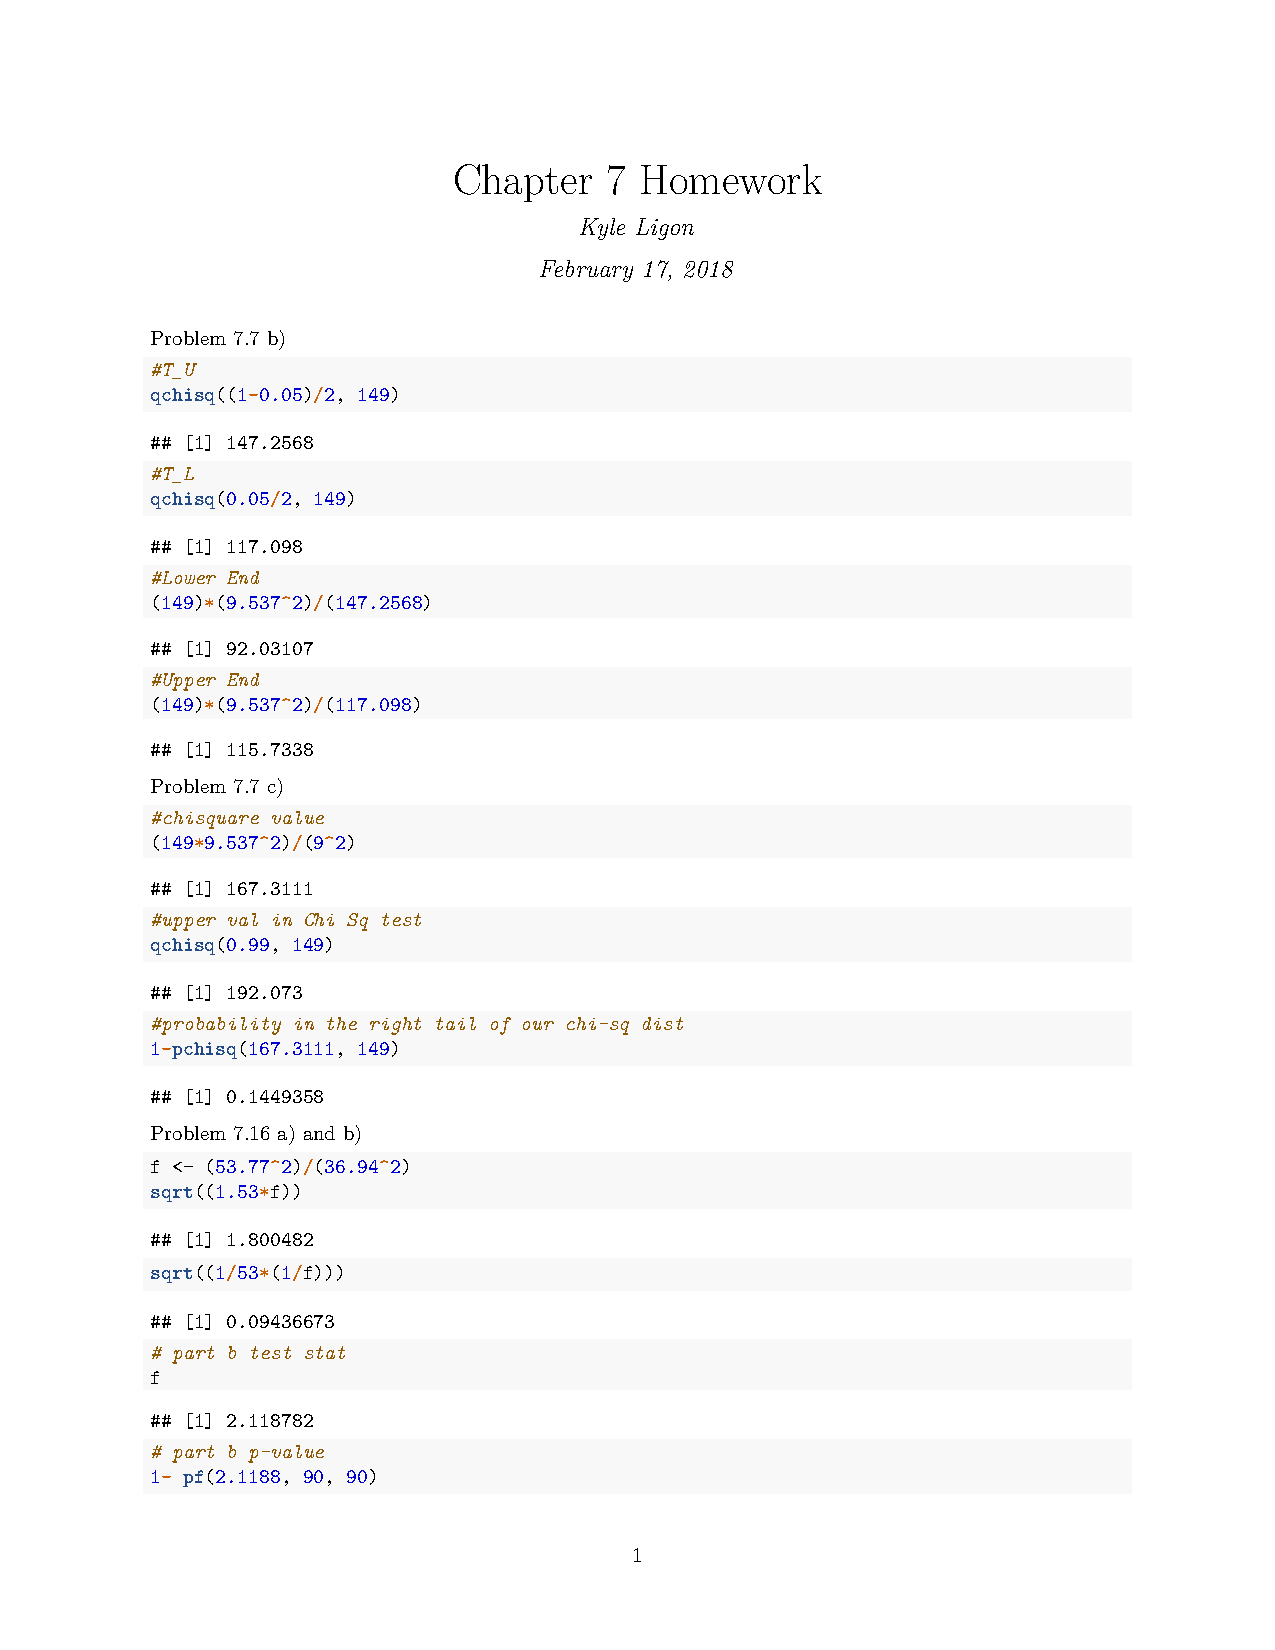
\includepdf[pages=-]{Chapter_7_Script.pdf}

\end{document}